\section{Nodecontroller}

\subsection{Data cache}

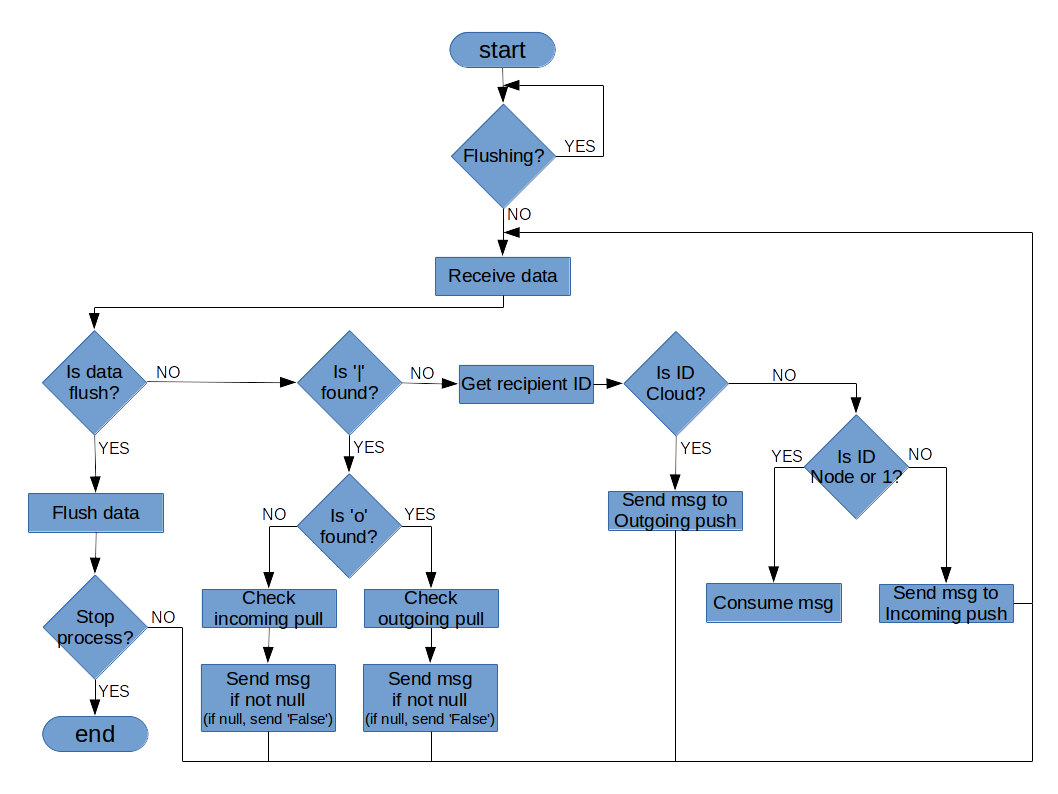
\includegraphics[width=\textwidth]{datacache_flowchart.png}

\textbf{TODO: data cache is consuming Waggle messages sent to the nodecontroller. We need to take the consumption part out from the data cache and put the part 
somewhere in internal communication.}

\subsection{Routing}
\label{routing}

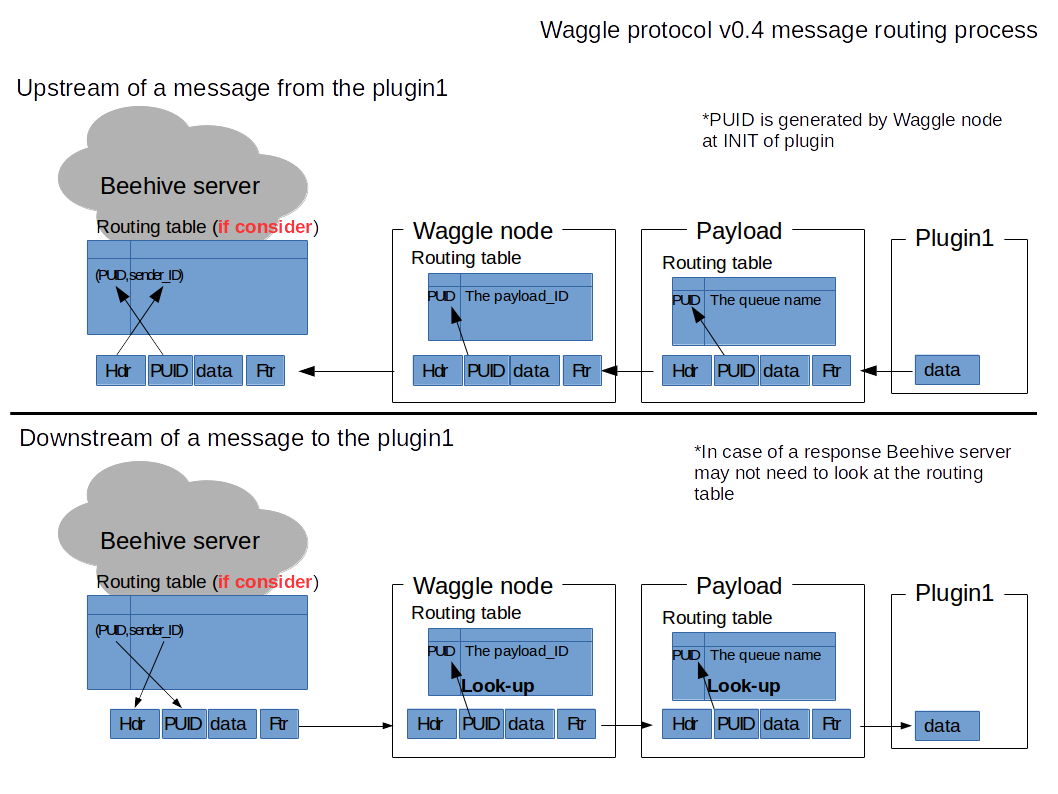
\includegraphics[width=\textwidth]{routing_process.png}

\noindent
Routing table is used to distribute Waggle messages to all connected components (i.e., payloads, plugins). All incoming Waggle messages 
that have $PUID$ in $Ext\_header$ set are consiered to be routed (Waggle messages that do not set $PUID$ are excluded for this route and will be 
consumed by the node). In the table, primary key is a unique number generated by nodecontroller and is mapped with routing information. An example of the 
routing table would look like,

\begin{center}
    \rowcolors{1}{rahmen!8}{white}
    \begin{tabular}{ | p{2cm} | p{3cm} | p{8cm} |}
    \hline
    \hline
    \textbf{ID} & \textbf{ROUTING} & \textbf{Meta} \\ \hline \hline
    0 & NODE\_ID & ``\{`name':`example\_plugin', `ver':`0.3', ... \}'' \\  \hline
    1 & PAYLOAD1\_ID & ``\{`name':`airsensor', `ver':`0.4', ... \}'' \\  \hline
    2 & PAYLOAD2\_ID & ``\{`name':`example\_plugin', `ver':`0.3', ... \}'' \\  \hline
    \end{tabular}
\end{center}

In this example ID 0 seems that it is a plugin attached to the nodecontroller. When a Waggle message with the ID 0 comes to the nodecontroller it will go to 
the `system\_receive' plugin running on the same node. ID 1 is also a plugin attached to the payload1 so the nodecontroller needs to send the message to the 
payload1 first and the message will be routed again in the payload1.

\subsubsection{Registration for routing}

The registration request ($Msg\_Mj\_Type$ `r' and $Msg\_Mj\_Type$ `r') will be sent to the parent node and will also be consumed at the node that has routing 
table. If the requestor is already in the routing table, a response message with the corresponding ID will be sent. When a registered plugin lost its 
ID or rebooted with a different instance a new ID will be assigned to the plugin. \textbf{TODO: we will need to clean up the routing table for some IDs that 
seem never used}

\subsubsection{Flushing the routing table to the server}

When the nodecontroller boots up it may wait until it gets a number of registration requests from attached plugins or payload nodes along with their meta data 
(e.g., name, version, instance, etc.). At a certain point of time, the nodecontroller needs to flush the routing table with all the meta data to the Beehive 
server so that the server could respond requests and sometimes send a message to the plugin registered in the routing table.

\subsubsection{Communication with Beehive server}

When connection is available to the server, nodecontroller pushes Waggle messages piled in the Data\_cache. All the outgoing Waggle messages will get the same
$S\_Uniq\_ID$ set by the ID of the nodecontroller so that the server only takes care of nodes, not plugins nor payloads.

